%
% $RCSfile: data_transfer_object.tex,v $
%
% Copyright (c) 2004. Christian Heller. All rights reserved.
%
% No copying, altering, distribution or any other actions concerning this
% document, except after explicit permission by the author!
% At some later point in time, this document is planned to be put under
% the GNU FDL license. For now, _everything_ is _restricted_ by the author.
%
% http://www.cybop.net
% - Cybernetics Oriented Programming -
%
% http://www.resmedicinae.org
% - Information in Medicine -
%
% @author Christian Heller <christian.heller@tuxtax.de>
%

\paragraph{Data Transfer Object}
\label{data_transfer_object_heading}

It is a well-known fact that many small requests between two processes, and
even more between two hosts in a network need a lot of time. A local machine
with two processes has to permanently change the \emph{Program Context}; a
network has a lot of \emph{Transfers}. For each request, there is a necessity
of at least \emph{two} transfers -- the \emph{Question} of the client and the
\emph{Answer} of the server.

Transfer methods are often expected to deliver common data such as a Person's
address, that is surname, first name, street, zip-code, town and so on. These
information is best retrieved by only \emph{one} transfer call. That way, the
client has to wait only once for a server response and the server does not get
too many single tasks. In this example, all address data would best be packaged
together and sent back to the client.

\begin{figure}[ht]
    \begin{center}
       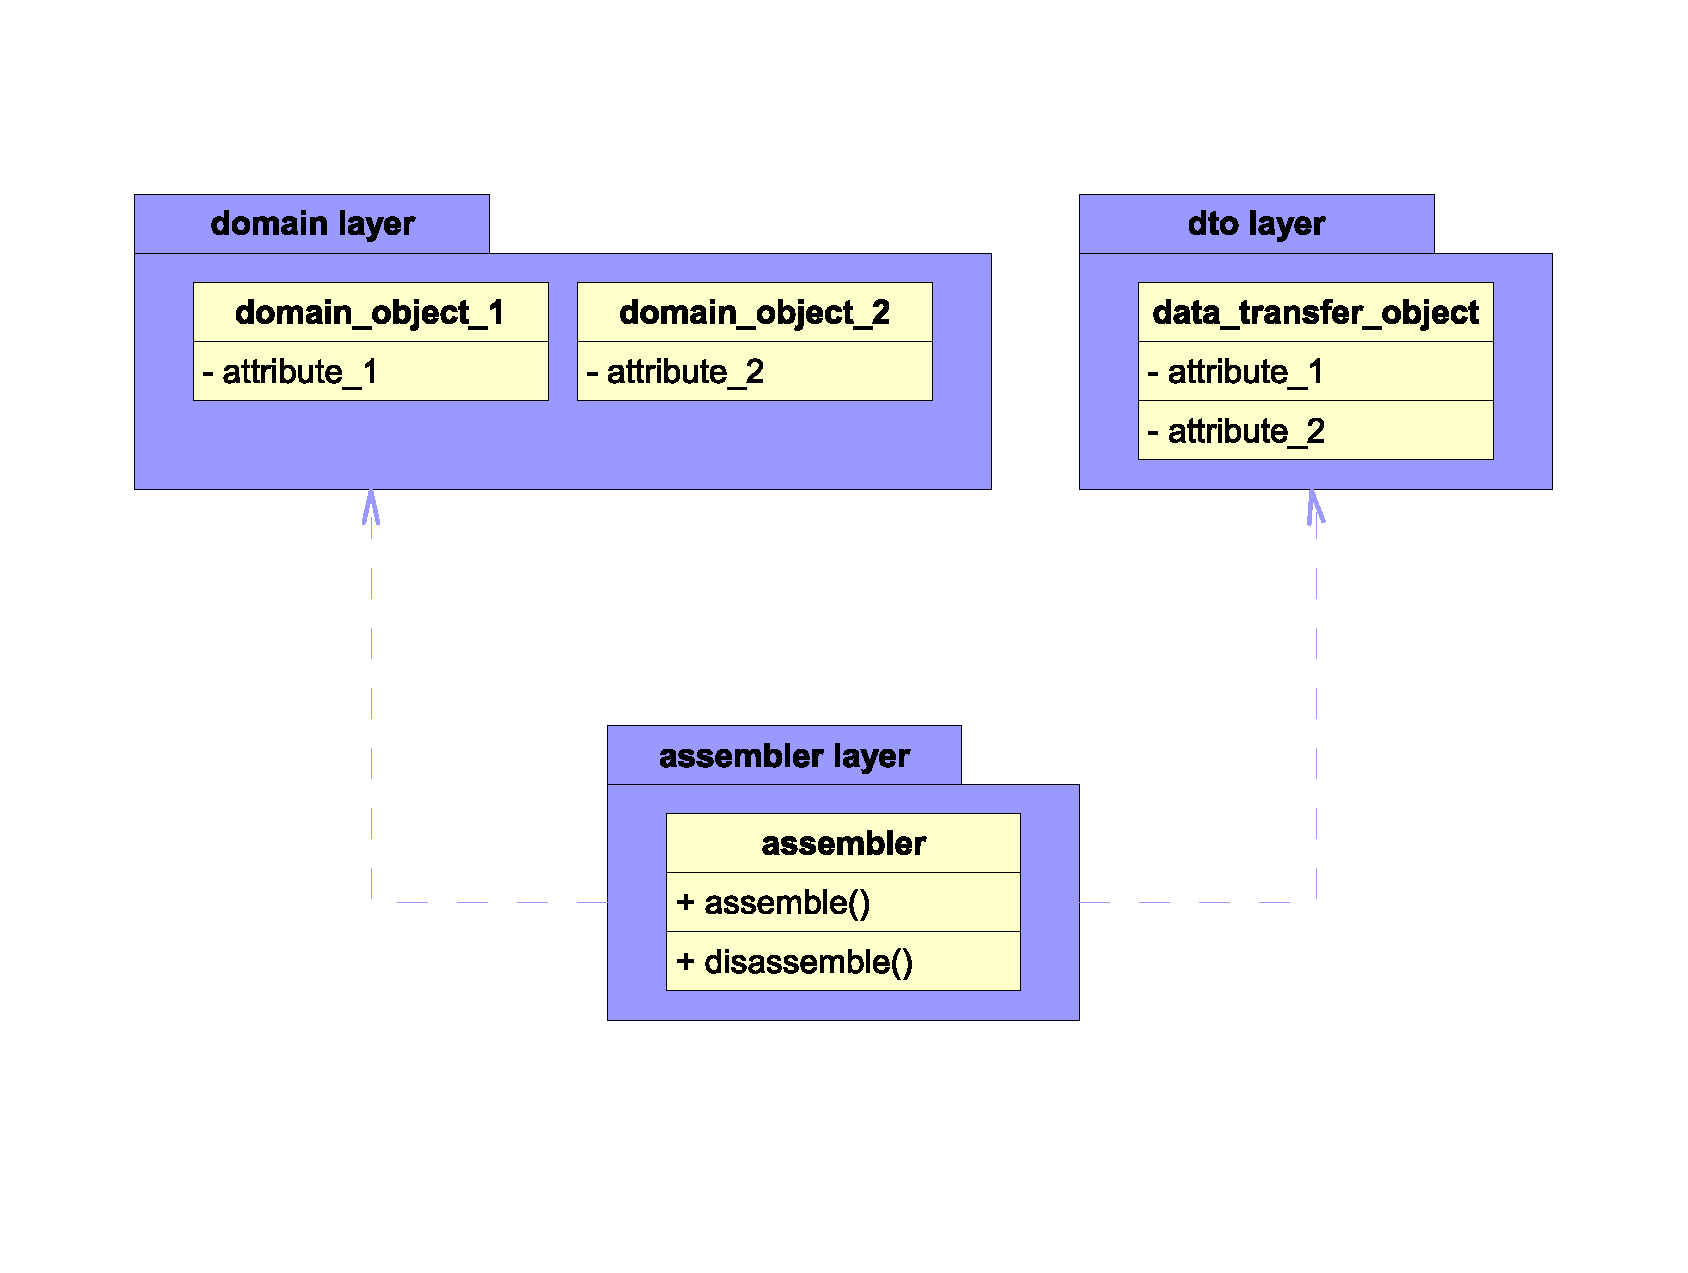
\includegraphics[scale=0.3]{vector/dto.eps}
       \caption{Data Transfer Object Pattern}
       \label{dto_figure}
    \end{center}
\end{figure}

A scenario of that kind is exactly what the \emph{Data Transfer Object} pattern
\cite{fowler2002} proposes a solution for: A central \emph{Assembler} object
takes all common data of the server's domain model objects and assembles them
together into a special \emph{Data Transfer Object} (DTO), which is a flat data
structure (figure \ref{dto_figure}). The server will then send this DTO over
network to the client. On the client's side, a similar assembler takes the DTO,
finds out all received data and maps (disassembles) them to the client's domain
model. In that manner, a DTO is able to drastically improve the communication
performance.
